\documentclass[11pt,a4paper]{article}

\usepackage[margin=2.4cm]{geometry}
\usepackage[T1]{fontenc}
\usepackage{lmodern}
\usepackage{microtype}
\usepackage{graphicx}
\usepackage{booktabs}
\usepackage{tabularx}
\usepackage{enumitem}
\usepackage{xcolor}
\usepackage{listings}
\usepackage{tikz}
\usetikzlibrary{positioning,arrows.meta,fit}
\usepackage[hidelinks]{hyperref}
\usepackage{caption}

\definecolor{accent}{HTML}{1D5C58}
\definecolor{codebg}{HTML}{F5F4EF}
\hypersetup{colorlinks=true,linkcolor=accent,urlcolor=accent}

\lstset{
  basicstyle=\ttfamily\small,
  backgroundcolor=\color{codebg},
  frame=single,
  rulecolor=\color{black!15},
  breaklines=true,
  columns=fullflexible,
  keepspaces=true,
  showstringspaces=false,
  keywordstyle=\color{accent}\bfseries,
  language=Java
}

\setlist{itemsep=2pt,topsep=4pt}
\captionsetup{font=small,labelfont=bf}
\graphicspath{{../}}

\title{\textbf{Advanced Programming, 2022}\\[4pt]
\large Report on the exercises and the final project}
\author{Alireza Astane\\[2pt]
\small Sharif University of Technology, Advanced Programming course (Dr.\ Tefagh)}
\date{Coursework written in 2022, completed and documented in November 2026}

\begin{document}
\maketitle

\begin{abstract}
\noindent
This report describes the Java work from the Advanced Programming course: three exercises with a design worth describing, a set of short algorithm exercises, and the final project. I wrote all of it in 2022, but two pieces were unfinished. In 2026 I returned to the repository, rebuilt the game from exercise~3 (\emph{Generals}) and the final project (\emph{Campus Portal}), and finished both. The report explains what each assignment asked for, how the original code was structured, what was changed and why, and how the result was tested and packaged. The 2022 code itself is kept unchanged in the \texttt{coursework} folder.
\end{abstract}

\tableofcontents
\newpage

%=====================================================================
\section{Overview}

\begin{table}[h]
\centering
\small
\begin{tabularx}{\textwidth}{@{}l X l@{}}
\toprule
\textbf{Folder} & \textbf{Content} & \textbf{State} \\
\midrule
\texttt{generals/} & A 5$\times$5 shogi-style board game (exercise 3), rewritten with a testable engine, a JavaFX interface and a computer opponent & Finished \\
\texttt{campus-portal/} & A university portal with a socket server and a JavaFX client (final project) & Finished \\
\texttt{coursework/} & Exercises 3 to 6 and the final project as left in 2022, with the assignment PDFs & Archive \\
\texttt{packaging/} & The script that turns an application into an AppImage & Tooling \\
\bottomrule
\end{tabularx}
\caption{Repository layout.}
\end{table}

Both active projects have their own Gradle build, their own README, and a GitHub Actions workflow that runs their tests on every push. A third workflow builds ready-to-run packages for Windows and Linux.

\subsection{Tools and technologies}

\begin{table}[h]
\centering
\small
\begin{tabularx}{\textwidth}{@{}l X@{}}
\toprule
\textbf{Tool} & \textbf{Where and why it is used} \\
\midrule
Java 21 & Language for every project. Records, switch expressions, text blocks and \texttt{var} are used where they make code shorter and clearer. \\
Gradle 9 & Build system, with the Gradle wrapper so that no separate installation is needed. The portal is a multi-project build with \texttt{common}, \texttt{server} and \texttt{client} modules. \\
JavaFX 21 & Desktop interfaces for Generals, the portal and exercise 4. The 2022 Generals used Swing. \\
Hibernate ORM 6 & Object-relational mapping for the portal server, using Jakarta Persistence annotations. \\
H2 and MariaDB & H2 is an embedded database used by default. MariaDB can be selected through a setting. \\
Gson & Serialises every message between portal client and server as one line of JSON. \\
BCrypt & Password hashing on the portal server. \\
Log4j 2 & Logging on server and client. \\
Lombok & Generates getters and setters for the portal's database entities. \\
JUnit 5 & Unit and integration tests. \\
Monocle & A headless JavaFX platform, so interface tests run without a screen, including on CI. \\
jpackage & Builds self-contained applications that carry their own Java runtime. \\
GitHub Actions & Runs the tests and builds Windows and Linux packages. \\
\bottomrule
\end{tabularx}
\caption{Tools used in the active projects.}
\end{table}

\begin{table}[h]
\centering
\small
\begin{tabular}{@{}lrr@{}}
\toprule
\textbf{Part} & \textbf{Main code (lines)} & \textbf{Test code (lines)} \\
\midrule
Generals & 1\,608 & 610 \\
Campus Portal server & 3\,634 & 709 \\
Campus Portal client & 3\,539 & 590 \\
Campus Portal shared module & 242 & -- \\
\bottomrule
\end{tabular}
\caption{Size of the rewritten projects.}
\end{table}

%=====================================================================
\section{Exercise 3: Game of Generals}

\subsection{The assignment}

The exercise asked for a 5$\times$5 variant of shogi (the assignment calls it \emph{Game of Generals}), playable both in a console and in a graphical window. Each side starts with a king, a golden general, a silver general, a bishop, a lance and one pawn. The rules that matter most are:

\begin{itemize}
\item Black moves first, pieces cannot jump, and capturing the enemy king wins. There is no check or checkmate.
\item Pawns, lances, bishops and silver generals upgrade when they end a move in the two rows nearest the enemy. Kings and golden generals never upgrade.
\item A captured piece changes sides, loses its upgrade, and goes to the capturer's hand. It can later be \emph{dropped} on any empty square, and a dropped piece is not upgraded on landing.
\item The console reads moves such as \texttt{p 54 53} (piece letter, origin, destination; upper case for White, \texttt{00} as origin for a drop) and prints the board, then each player's hand, after every line. Illegal moves leave the state unchanged.
\end{itemize}

\subsection{The 2022 implementation}

The original program (\texttt{coursework/exercise\_3/src.zip}) has a \texttt{Logic} package with one class per piece, a \texttt{Movementcmd} for a parsed move, a \texttt{Rule} class that checks legality, and a Swing \texttt{GameFrame} that places buttons at fixed pixel positions over a board image. Each piece class returns a list of displacement vectors, which \texttt{Rule} compares with the requested move and then checks for blocking pieces along the path.

It follows the console format of the assignment, but all game state lived in \emph{static} fields of \texttt{Game}. That made it impossible to copy a position, which a computer player needs, and hard to test pieces in isolation.

\subsection{The rewritten engine}

The engine in \texttt{generals/src/main/java/generals/logic} keeps the original vocabulary (sides, piece types, moves) but holds all state in a \texttt{Game} object that can be copied.

\begin{itemize}
\item \textbf{Movement as data.} Each \texttt{PieceType} lists its \emph{steps}: a direction written from White's point of view and a range (one square, two squares, or any distance). Black's moves are the same steps multiplied by $-1$. Upgraded pieces use a second table, so a promoted lance is simply ``four straight directions, any distance''.
\item \textbf{Move generation.} \texttt{targets(square)} walks along each step until it leaves the board or meets a piece. A friendly piece stops the walk; an enemy piece is included and then stops it. \texttt{legalMoves()} adds every drop of each distinct hand piece onto every empty square.
\item \textbf{Applying a move.} \texttt{play(move)} validates and applies. \texttt{after(move)} returns a new position and is used by the search, which explores thousands of positions per second.
\item \textbf{Console.} \texttt{Main} parses the original input format and prints the original output format, so the console behaves exactly as the assignment required.
\end{itemize}

\subsection{Verifying the rewrite against the 2022 program}

The 2022 program is the version I submitted, so it serves as the reference for the rules. Two techniques were used:

\begin{enumerate}
\item \textbf{Recorded transcripts.} Forty random games, mixing legal moves, captures, drops and deliberately malformed lines, were played through the original program and its output stored. A parameterised test replays all forty against the new console and requires identical output.
\item \textbf{Differential testing of illegal moves.} Recorded games only test moves the new engine accepts. To catch moves it wrongly \emph{rejects}, a one-off comparison generated, at every turn of 25 more games, every move the new engine considered illegal (339\,680 probes) and fed them to both programs. They agreed on every one.
\end{enumerate}

In addition, 67 automated tests cover each piece's movement, blocking, promotion, demotion on capture, drops, king capture and the interface. A deliberate mutation (promoting one row too early) is caught by the rule tests.

\subsection{The computer player}

\texttt{generals.ai.Computer} uses \textbf{negamax search with alpha-beta pruning}.

\begin{itemize}
\item \textbf{Evaluation.} Material counted from the side to move, using a value per piece type that rises when the piece is upgraded. Pieces in hand count slightly more than on the board, because a drop can land anywhere. Each piece also adds a little for every square it can reach, which rewards activity.
\item \textbf{Wins.} Capturing the king scores close to infinity, reduced by the distance from the root, so the search prefers faster wins and slower losses. At depth zero, a position where the side to move can capture the enemy king is scored as a win immediately.
\item \textbf{Move ordering.} Captures are searched first, biggest victim first, so that pruning happens early.
\item \textbf{Levels.} \emph{Easy} searches one ply and adds random noise to the score; \emph{Normal} searches three plies with small noise; \emph{Hard} uses iterative deepening for about 1.2 seconds and keeps the best move of the deepest finished iteration.
\end{itemize}

A test plays twelve games of Normal against Easy and requires Normal to win at least ten.

\subsection{The interface}

\begin{figure}[h]
\centering
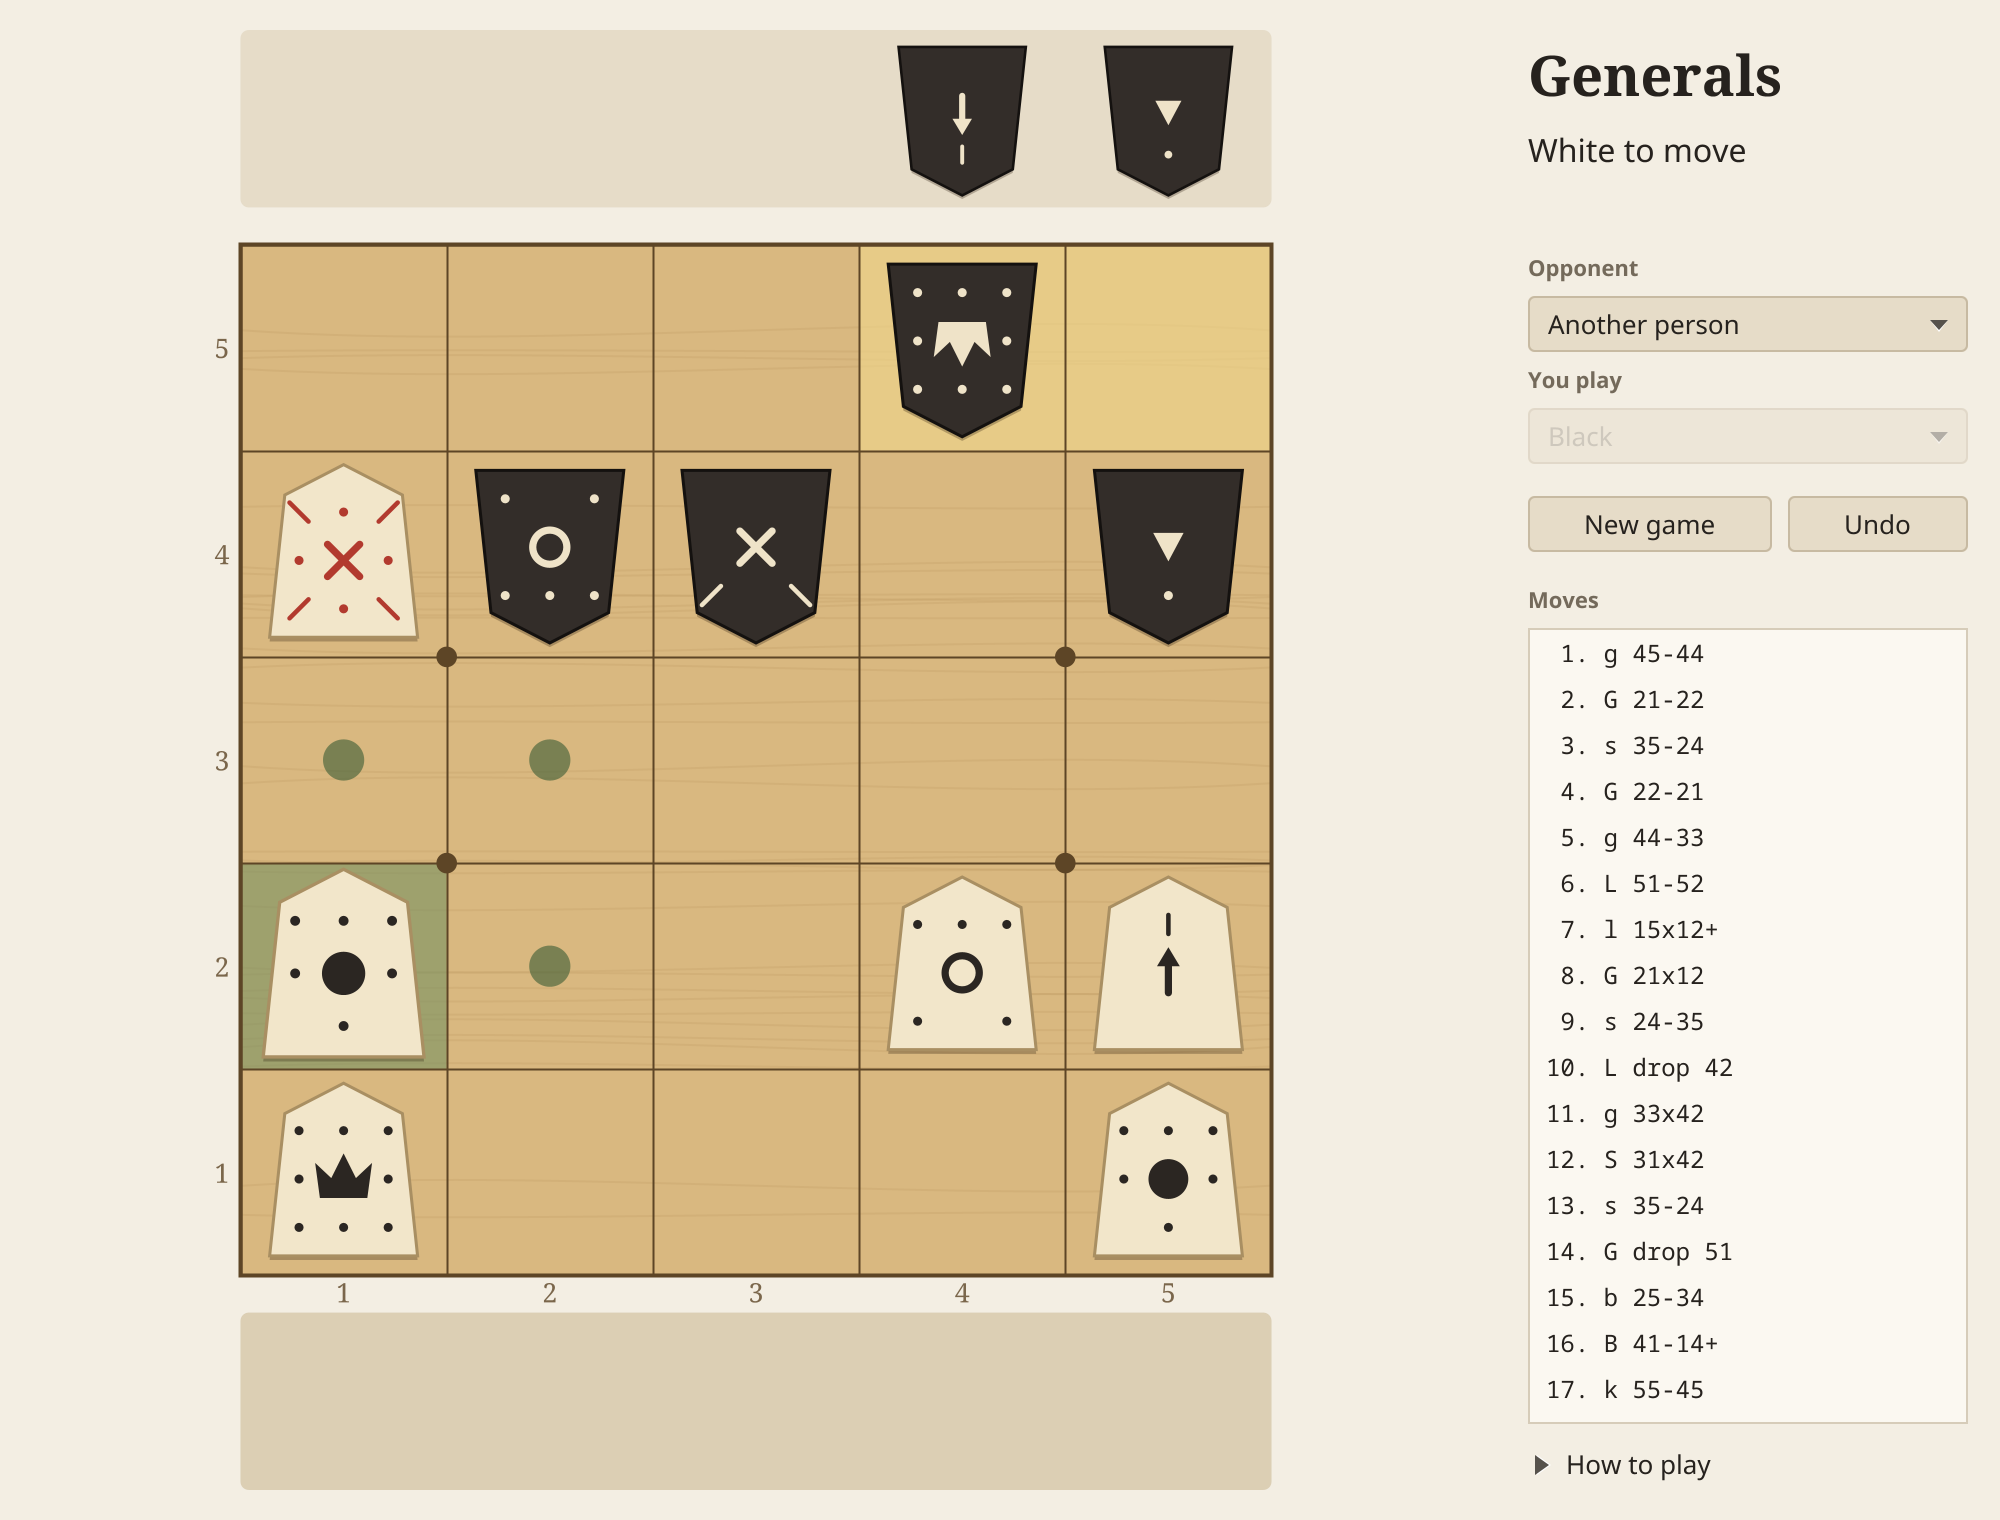
\includegraphics[width=0.82\textwidth]{generals/docs/board.png}
\caption{Generals during a game. The marks on each tile show how that piece moves; red marks mean the piece is upgraded.}
\end{figure}

The Swing window was replaced by JavaFX. The board and both hands are painted on one \texttt{Canvas}, so a piece can slide from a hand to the board in the same animation. Pieces are five-sided tiles drawn in code, pointing the way they advance, with a small symbol and \emph{movement marks}: a dot for one step, two dots for two steps, a line for any distance. Upgraded pieces have red marks. The original piece images, whose source I could not confirm, are no longer used.

Players can click or drag. Legal targets are highlighted, the last move is shaded, a king that can be captured is framed in red, and there are a move list, undo and new game. The computer thinks on a background thread; a counter discards its answer if the user starts a new game or undoes while it is thinking.

The interface is tested headlessly with Monocle: tests send real mouse events to the canvas and check the resulting game state, including drops from the hand, undo against the computer and the end of the game.

%=====================================================================
\section{Exercise 4: Coup simulator}

The exercise asked for a JavaFX simulation of the card game \emph{Coup} for one human and three computer players. The 2022 code (\texttt{coursework/exercise\_4/code.zip}) is kept as it was and was not developed further, because the result would be a recreation of a commercial game.

\subsection{Design}

\begin{itemize}
\item \textbf{Actions as classes.} An abstract \texttt{Action} knows its actor, target, the card it claims, and whether it can be challenged or blocked. Subclasses implement \texttt{Income}, \texttt{ForeignAid}, \texttt{Tax}, \texttt{Steal}, \texttt{Assassinate}, \texttt{Exchange}, \texttt{Coup} and the blocking actions. Resolving a challenge checks whether the actor really holds the claimed card, and the loser of the challenge gives up a card.
\item \textbf{Strategies as players.} The bots are subclasses of \texttt{Player} that override \texttt{act()} and the \texttt{react\_to\_\ldots} methods:
\begin{itemize}
\item \emph{Coup Maker} collects tax and launches a coup as soon as it has seven coins;
\item \emph{Paranoid} takes income until it can afford a coup;
\item \emph{Coward Communist} steals from the richest player and never challenges;
\item \emph{Cautious Assassin} assassinates when it holds the right card and can pay, otherwise plays safe.
\end{itemize}
Each bot blocks assassinations when it holds the blocking card, and otherwise occasionally bluffs a block.
\item \textbf{Configuration.} The starting hands and player types are read from a JSON file with Gson, so a game can be set up without changing code.
\item \textbf{Interface.} An FXML layout with card images, a coin count per player, a step button that advances the bots, and a history table of events. Challenges and blocks open dialogs for the human player.
\end{itemize}

%=====================================================================
\section{Exercise 5: Data structures}

Exercise 5 is a set of short console programs, kept in \texttt{coursework/exercise\_5}. Each reads its input from standard input in the format set by the course's automatic judge.

\begin{description}[style=nextline]
\item[Sparse matrix addition (\texttt{Main (1).java})]
Each matrix row is a \texttt{LinkedList} of \texttt{(column, value)} pairs, so only non-zero entries are stored. Adding two matrices merges the two lists of each row, sums the values of equal columns, and sorts the result by column with a \texttt{Comparator}.

\item[Matrix operations (\texttt{Main (2).java})]
Matrices are lists of lists. The program multiplies two matrices, transposes, computes the trace and a norm, selected by a one-letter command. Dimension mismatches print an error instead of failing.

\item[Rearranging a train with stacks (\texttt{Main (3).java})]
Wagons $1\ldots n$ wait on a western track and must reach the eastern track in a given order, using one siding. All three tracks are stacks, and the program prints the moves (west to siding, west to east, siding to east). The algorithm is greedy: if the wagon needed next is on top of the siding, move it east; otherwise park wagons from the western track on the siding until the needed wagon is on top, then send it east. If the needed wagon is already buried, the order is impossible and the program prints $-1$.

\item[Collections (\texttt{Main (4).java})]
Reads either an \texttt{ArrayList} of numbers or a \texttt{LinkedHashMap} of key-value pairs and applies a named operation: insert, contains, contains key, get index, get size, get value, modify, or extract, reverse and rejoin a sub-list. Each operation is a small static class with a \texttt{perform()} method.
\end{description}

%=====================================================================
\section{Exercise 6: The Mind (unfinished)}

The assignment asked for a networked version of the cooperative card game \emph{The Mind}: clients connect to a server, a host chooses the number of players, the server fills empty seats with bots that wait a time based on their lowest card, and players can send emoji reactions. Every message had to carry an authentication token created with \texttt{SecureRandom}.

The 2022 code (\texttt{coursework/exercise\_6/TheMind.zip}) contains the communication layer:
\begin{itemize}
\item \texttt{ClientMessage} and \texttt{ServerMessage} types, serialised with Gson, one per line;
\item a \texttt{ClientHandler} thread per connection on the server;
\item receiver and messenger classes that decode messages and dispatch on their type.
\end{itemize}
The game rules and the bots were never written, and the code does not compile because of unfinished \texttt{switch} branches. It is kept as an archive and was not continued, again because it would recreate a commercial game. The ideas tried here (one thread per client, a token per connection, one JSON message per line) were used for the final project.

%=====================================================================
\section{Final project: Campus Portal}

\subsection{The assignment}

The project was given in two phases (\texttt{coursework/Project/phase1.pdf} and \texttt{phase2.pdf}). Together they describe a copy of the university's education and courseware systems:

\begin{itemize}
\item accounts for students at three levels, professors, department deputies, heads of department, a registrar and an administrator, with a picture captcha, hashed passwords and a forced password change after more than three hours away;
\item course and professor lists with filters, and management of courses and professors by department staff;
\item weekly plans, exam lists, and requests: recommendation letters, enrollment certificates, minors, withdrawal, dormitory and dissertation defense;
\item temporary and final grades with objections, and academic records;
\item unit selection within time windows, with capacity, prerequisite and time-clash rules;
\item an inbox of requests and notices, and a messenger with files;
\item courseware with learning content, exercises, answers and a calendar;
\item a client-server architecture over sockets, automatic refresh, an offline mode, and a database.
\end{itemize}

The full checklist, with every item marked, is in \texttt{campus-portal/docs/REQUIREMENTS.md}.

\subsection{State of the 2022 version}

The 2022 version is large (about 16\,000 lines and 64 screens) but was never finished. Reviewing and running it showed:
\begin{itemize}
\item the login accepted any password, because it compared strings with \texttt{==};
\item several screens could not open because their layouts referenced missing handlers, and many buttons had no code;
\item the data layer looked records up with the wrong key types, read related data after its database session had closed, and shared one session between all clients;
\item automatic refresh was switched off and offline mode was incomplete;
\item it depended on Log4j 2.14.1, which has a critical vulnerability, and on file paths of the original Windows machine.
\end{itemize}
Because these problems ran through the data layer and the client-server protocol, both were rebuilt rather than patched. The domain model and vocabulary (users, masters, students, courses, scores, university requests) were kept.

\subsection{Architecture}

\begin{figure}[h]
\centering
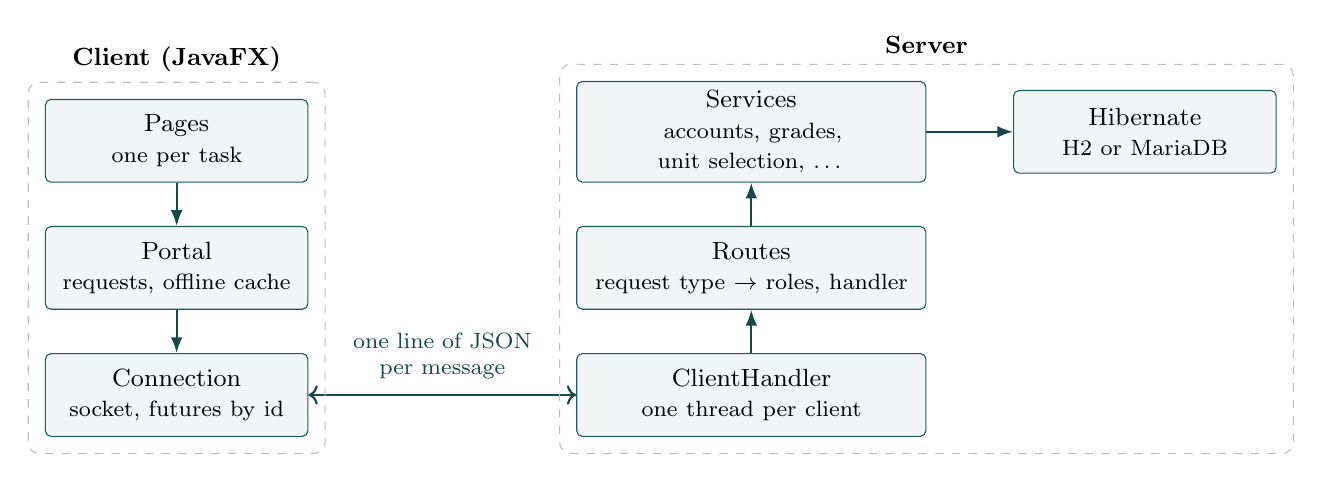
\begin{tikzpicture}[
  box/.style={draw=accent, rounded corners=2pt, fill=accent!6, align=center, minimum height=1.05cm, text width=3.1cm, font=\small},
  wide/.style={box, text width=4.2cm},
  arrow/.style={-{Latex[length=2mm]}, thick, accent!80!black},
  node distance=0.55cm and 1.1cm]
\node[box] (pages) {Pages\\{\footnotesize one per task}};
\node[box, below=of pages] (portal) {Portal\\{\footnotesize requests, offline cache}};
\node[box, below=of portal] (conn) {Connection\\{\footnotesize socket, futures by id}};
\node[wide, right=3.4cm of conn] (handler) {ClientHandler\\{\footnotesize one thread per client}};
\node[wide, above=of handler] (routes) {Routes\\{\footnotesize request type $\to$ roles, handler}};
\node[wide, above=of routes] (services) {Services\\{\footnotesize accounts, grades, unit selection, \ldots}};
\node[box, right=1.1cm of services] (db) {Hibernate\\{\footnotesize H2 or MariaDB}};
\draw[arrow] (pages) -- (portal);
\draw[arrow] (portal) -- (conn);
\draw[arrow, <->] (conn) -- node[above=2pt, font=\footnotesize, align=center, text width=2.3cm]{one line of JSON per message} (handler);
\draw[arrow] (handler) -- (routes);
\draw[arrow] (routes) -- (services);
\draw[arrow] (services) -- (db);
\node[draw=black!25, dashed, rounded corners, fit=(pages)(conn), inner sep=6pt, label={[font=\small\bfseries]above:Client (JavaFX)}] {};
\node[draw=black!25, dashed, rounded corners, fit=(handler)(services)(db), inner sep=6pt, label={[font=\small\bfseries]above:Server}] {};
\end{tikzpicture}
\caption{How a request travels from a page to the database and back.}
\end{figure}

The build has three modules:
\begin{itemize}
\item \textbf{common} holds the message format: \texttt{Request} (type, arguments, optional file), \texttt{Response} (named values, named tables of rows, optional file, or an error) and \texttt{Protocol} (the Gson configuration and a line reader with a size limit).
\item \textbf{server} accepts connections, routes requests, and owns the database.
\item \textbf{client} is the JavaFX application.
\end{itemize}

\subsection{Protocol}

Every message is one line of JSON. Files travel inside messages as Base64, and lines longer than the limit for a 20\,MB file are rejected, so a client cannot exhaust server memory. Each request carries a \emph{request id}, which the response repeats; the client keeps a map from id to a \texttt{CompletableFuture}, so several pages can wait for answers at the same time without mixing them up. Messages with id~0 come from the server unprompted: the connection's authentication token, and a warning when the server loses its database.

Each connection receives a 256-bit token from \texttt{SecureRandom}, and requests with another token are ignored. After login the client also receives a \emph{session key}, which lets it resume after a dropped connection without logging in again.

\subsection{Routing and access control}

Each service registers its request types in one place, together with the roles allowed to send them:

\begin{lstlisting}
routes.on(RequestType.SET_SCORE, Routes.STAFF, ScoreService::setScore);
routes.on(RequestType.TAKE_COURSE, Routes.STUDENT, UnitSelectionService::take);
routes.open(RequestType.LOGIN, AccountService::login);
\end{lstlisting}

The \texttt{ClientHandler} refuses a request before it reaches a handler if nobody is logged in, if the password has expired (only a password change is allowed then), or if the user's role is not listed. Handlers then check \emph{ownership}: a professor may grade only their own course, a deputy may change only their own department's courses, a chat can be read only by its members, and a request can be answered only by the person it was sent to. Refusals raise a \texttt{Problem} exception whose message is shown to the user.

\subsection{Data model and transactions}

The database has thirteen entities: users, departments, masters (professors), students, courses, scores, university requests, chats, messages, course content, content items, exercises and answers, plus a table for uploaded files. Relations are real foreign keys: a score belongs to a course and a student, a course to a department and a professor, and enrolment, teaching assistance, course selection and starred courses are many-to-many join tables. Uploaded files live in their own table and are loaded lazily, so listing messages never loads their attachments.

Every request runs in \textbf{one database transaction} on its own session, held in a \texttt{ThreadLocal}. Entities stay attached while a response is built, and if a handler throws, the transaction is rolled back, so a refused or failed request changes nothing. Several clients are served at once, each on its own thread and session.

\subsection{Security}

\begin{itemize}
\item Passwords are hashed with BCrypt and are never sent to any client.
\item Captchas are generated on the server as distorted PNG images of a random four-digit code, and each code works only once.
\item A login is refused with the same message whether the username or the password was wrong.
\item Log4j and all other libraries were updated to current versions.
\end{itemize}

\subsection{Features and the rules behind them}

\paragraph{Grades.} A score passes through three states. While a professor enters values, students see nothing. Grades must be between 0 and 20 and are rounded to the nearest 0.25. Temporary publication is allowed only once every student has a grade; students can then object, and the professor can answer and change the grade. Final publication locks the grades and moves them to the academic record, where the average is weighted by course units. Deputies see every published grade of their department with filters, and a summary per course: average, number passed and failed, and the average of those who passed.

\paragraph{Unit selection.} The menu appears only during a student's window, which the deputy sets by level and entry year. Taking a course checks, in order: the student's level, whether the course (or another group of it) is already taken or passed, prerequisites, exam clashes, class clashes, the single general-course rule, the unit limit, and capacity. Class times are parsed from strings such as \texttt{Sun 09:00-10:30} and two meetings clash when they share a day and their intervals overlap. A full course or full group can be requested from the deputy, who accepts or rejects it in the inbox.

When a window closes, a background task \emph{confirms} each student's choices. Courses whose prerequisites were not passed, or whose corequisites are not also kept, are removed, and the check repeats until nothing changes, because one removal can invalidate another course. The remaining courses become enrolments with empty scores and course pages, and the student receives a notice for each course kept or dropped.

\paragraph{Requests.} Requests are stored with their requester and the person responsible. A minor needs a minimum average and the approval of both the student's own deputy and the target department's deputy: it is accepted only when both agree, and rejected as soon as one refuses. An accepted withdrawal changes the student's status and blocks their login. A recommendation letter is written from the student's passed and assisted courses when the professor accepts it. Dormitory requests are decided at random, as the assignment asks.

\paragraph{Messenger.} Chats are sorted by their last message and can carry files. Who may write to whom follows the assignment: students reach classmates of the same department and year and their supervisor, professors reach their advisees, heads and deputies reach their department, and the registrar and administrator reach everyone. A message to someone outside that list starts as a chat request. Support messages go to the administrator, the account with user id~1.

\paragraph{Courseware.} Professors create learning content with up to five text or file items, and exercises with opening, free-submission and closing times and an answer type. Teaching assistants can edit items and grade answers, but they cannot create or delete anything, and they see students' names and numbers masked with asterisks.

\subsection{The client}

\begin{figure}[h]
\centering
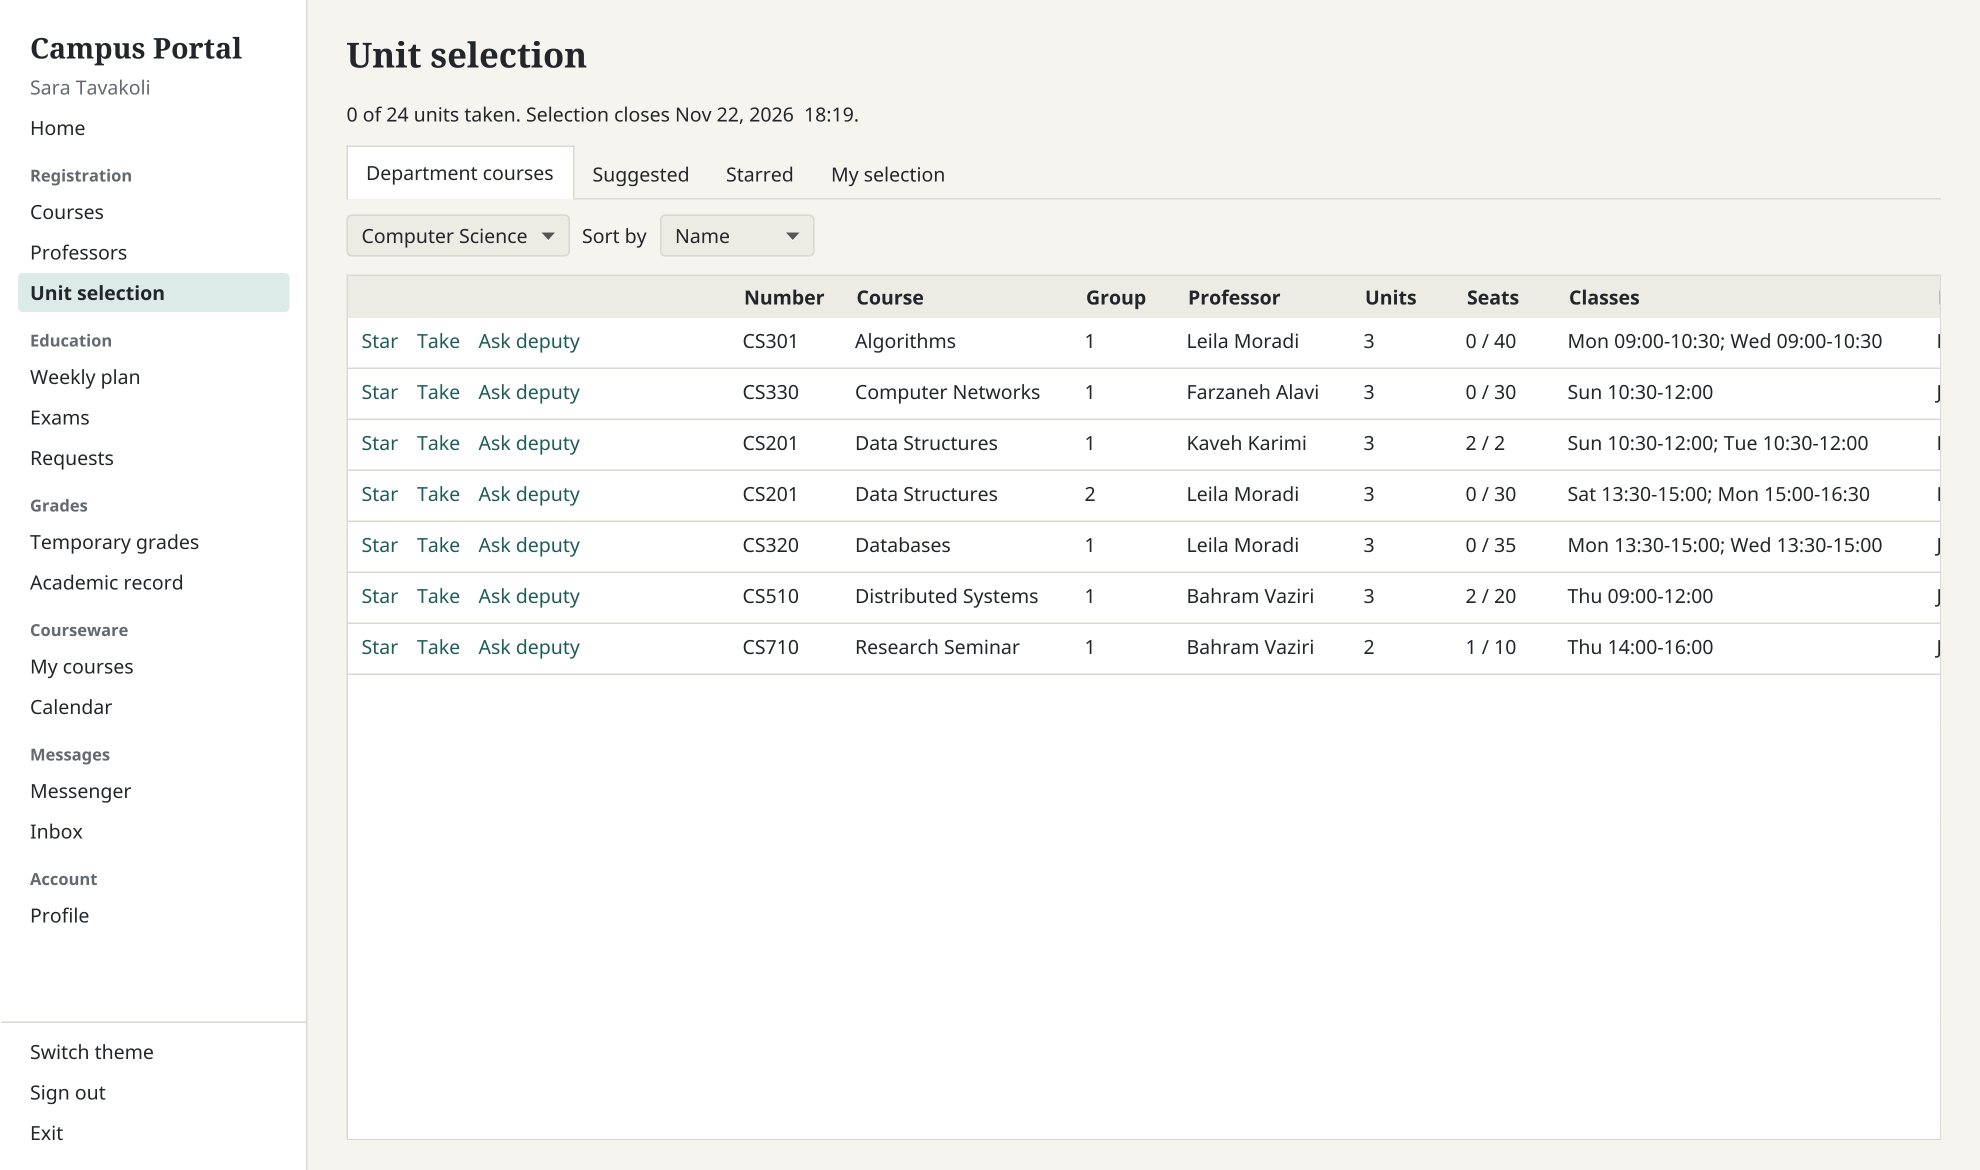
\includegraphics[width=\textwidth]{campus-portal/docs/screens/student-sara-unit-selection.png}
\caption{Unit selection as a student. Row actions come first, so they stay in view when the table scrolls sideways.}
\end{figure}

The client has one window with a sidebar that lists the pages a role can use, a page header, and a content area. Each page is a small class that knows how to load its data and render it; most are a filtered table built from a reusable \texttt{DataTable} that sizes its columns to their content. Forms are shown in dialogs that stay open with the server's error message if a request is refused.

\begin{itemize}
\item \textbf{Automatic refresh.} The visible page reloads every four seconds, as the assignment forbids a refresh button. Tables keep their selection, and filters and forms are never overwritten.
\item \textbf{Offline mode.} Home, profile, weekly plan, exams, academic record, the chat list and the last ten messages of each chat are saved on disk whenever they load. If the connection drops, a banner appears, saved pages still open, other pages say they are unavailable offline, and support messages are queued and sent after reconnecting. The client can also be started offline to read the last user's saved pages.
\item \textbf{Themes.} Colours are defined once as variables in the stylesheet, with a light and a dark set; the theme switch swaps them.
\item \textbf{Demo server.} If no server is reachable, the login screen can start one inside the client, with demo data, so a single download is enough to try the portal.
\end{itemize}

\begin{figure}[h]
\centering
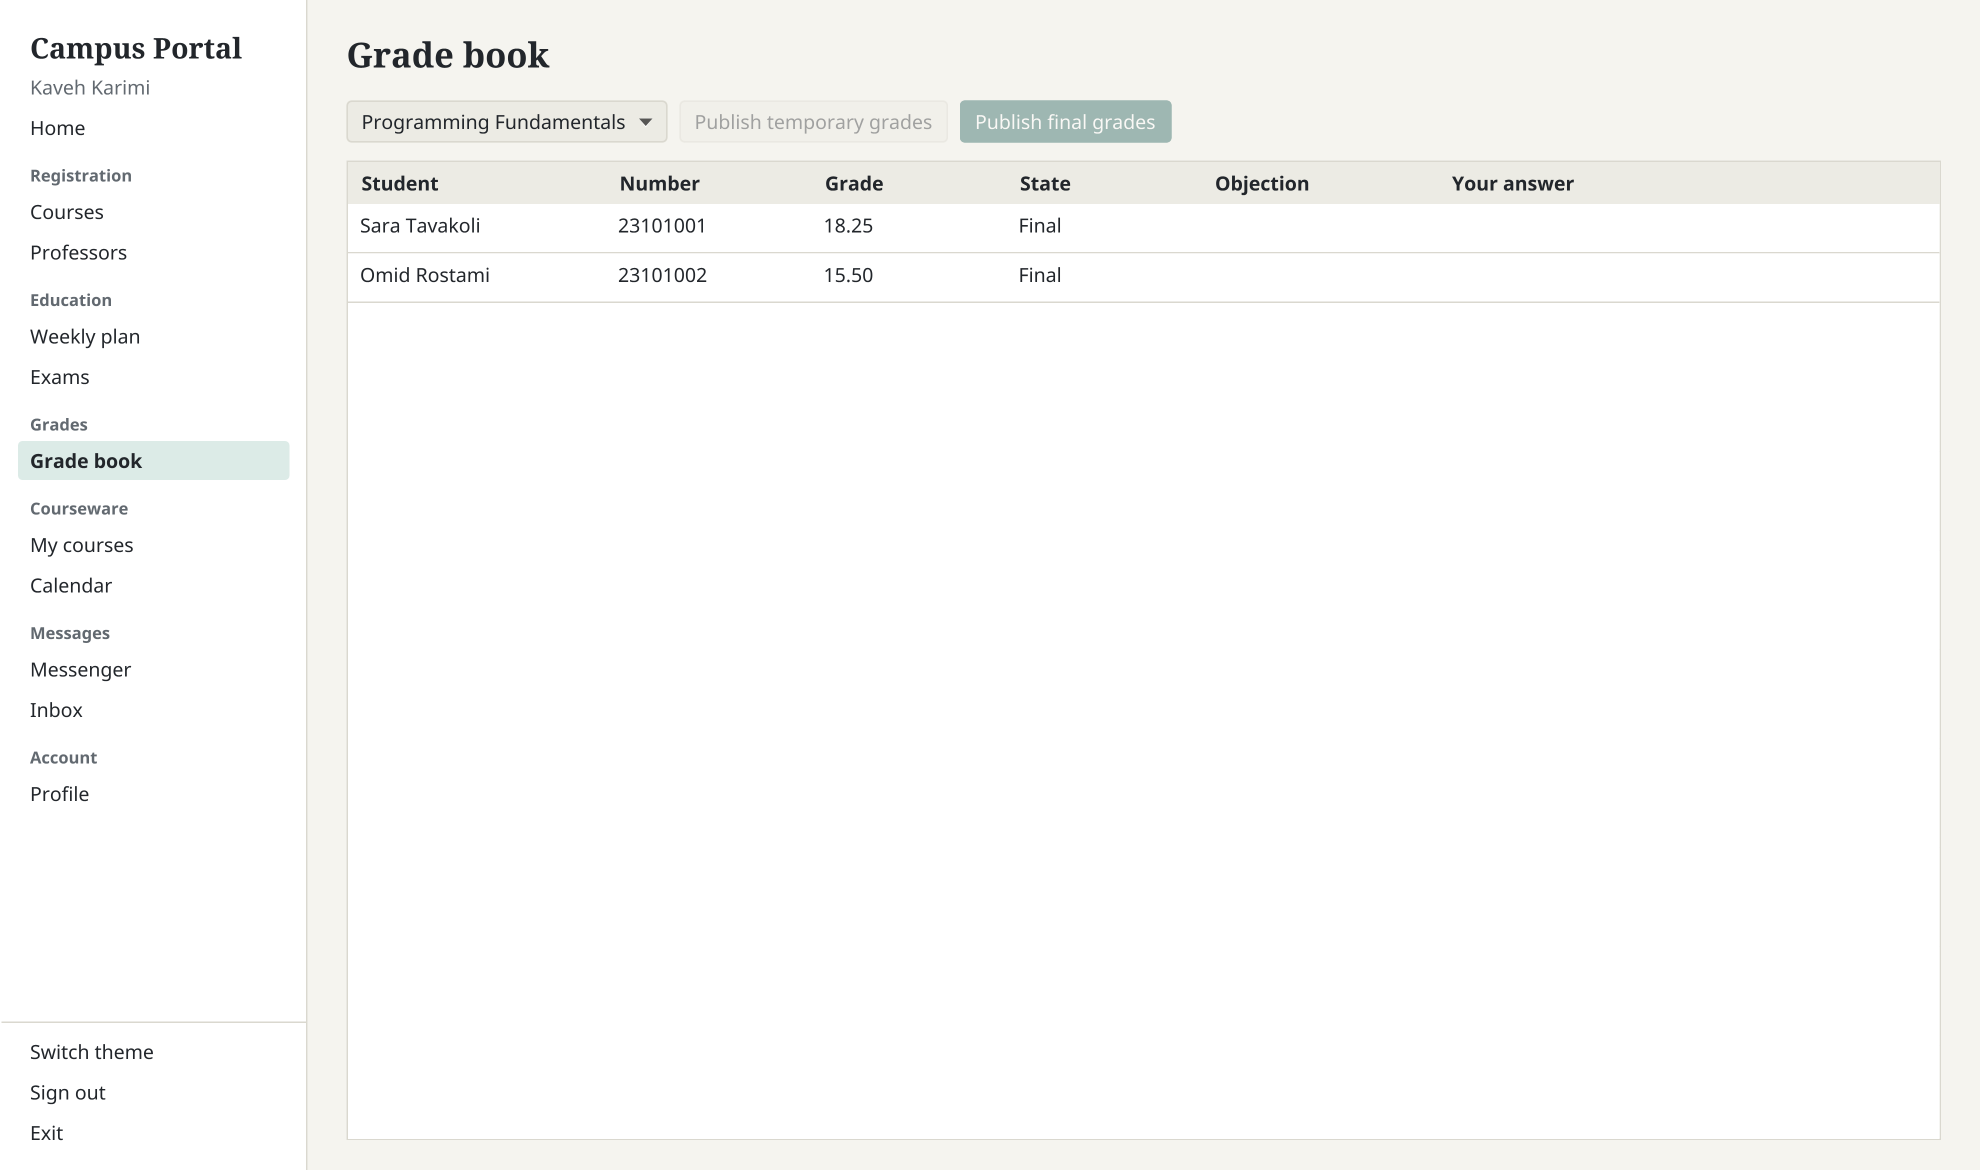
\includegraphics[width=0.49\textwidth]{campus-portal/docs/screens/prof-karimi-grade-book.png}\hfill
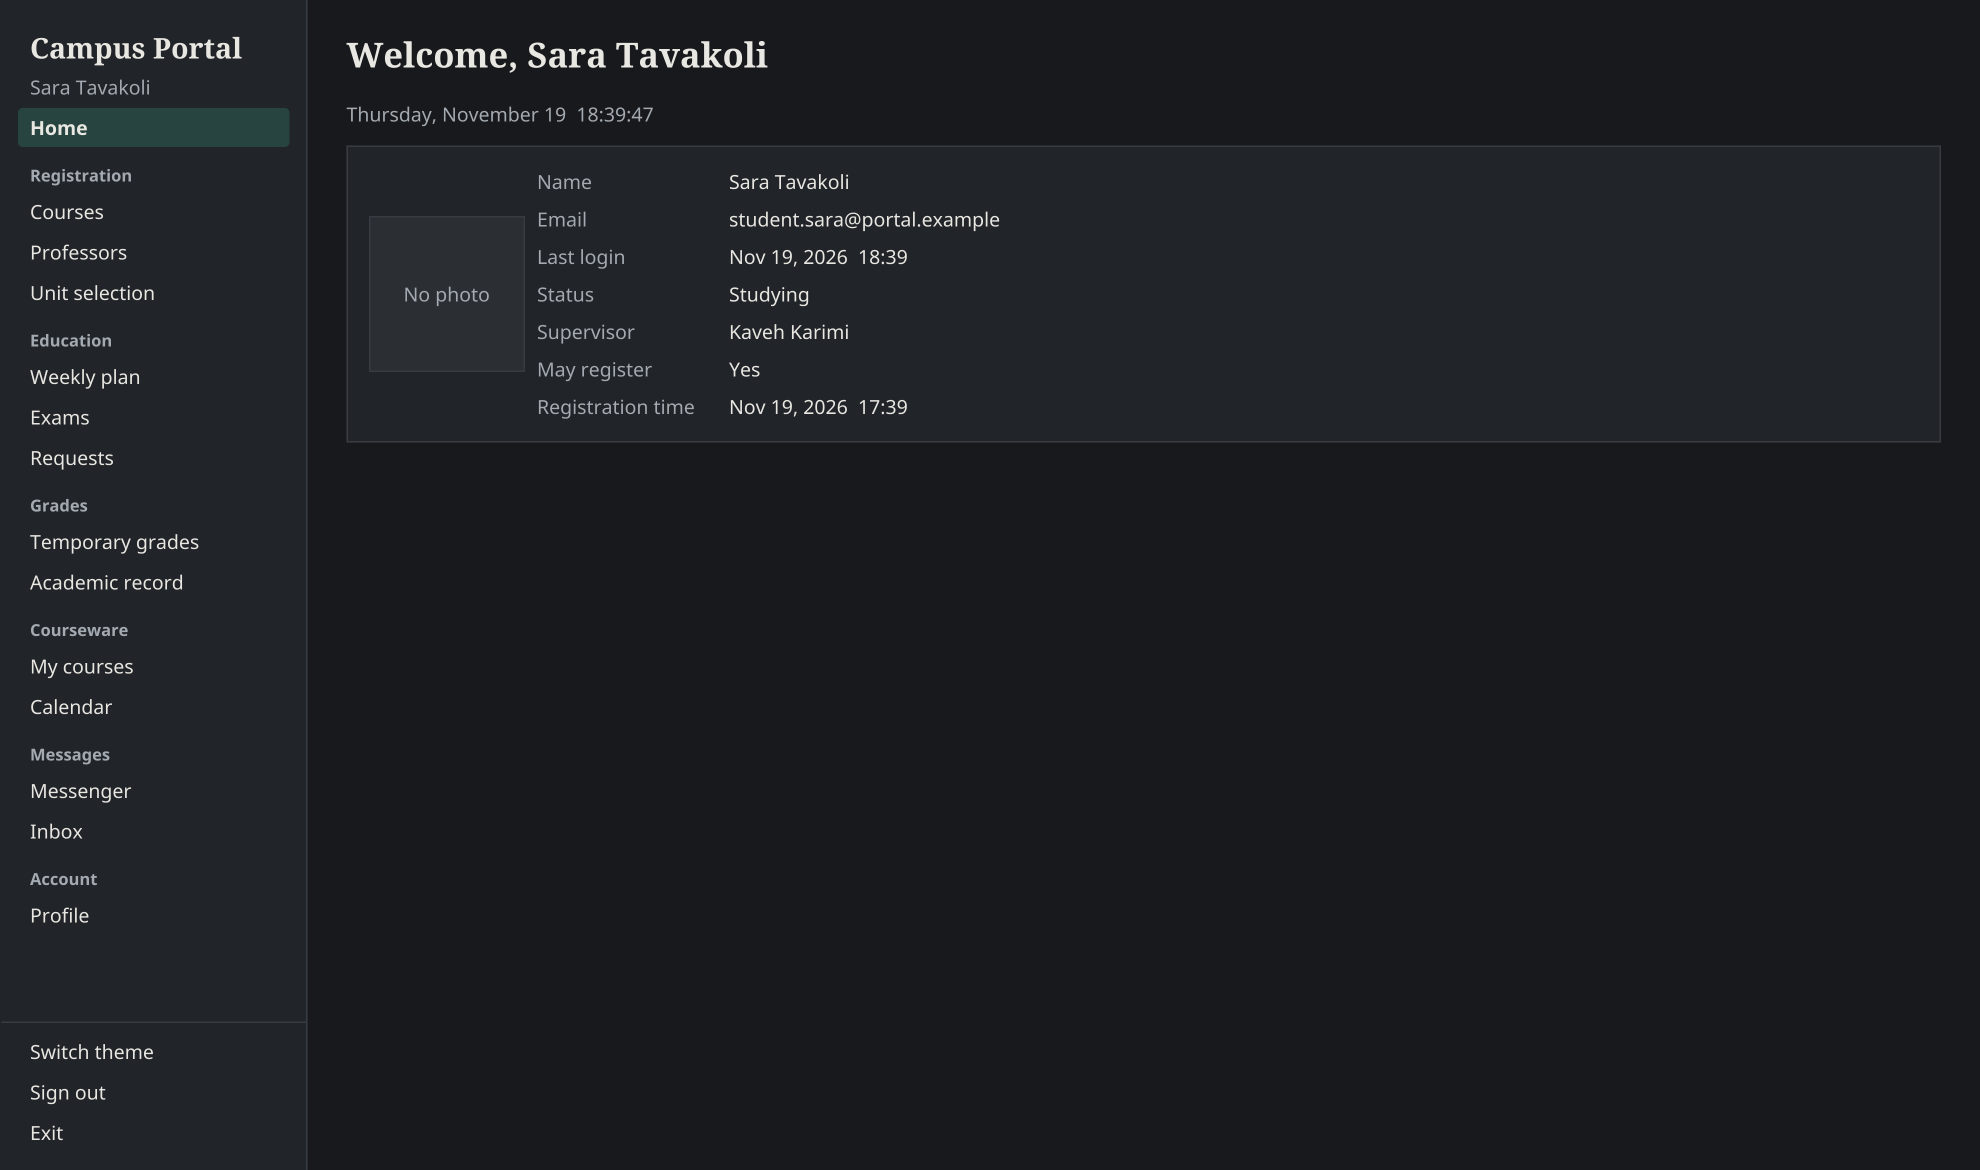
\includegraphics[width=0.49\textwidth]{campus-portal/docs/screens/dark-home.png}
\caption{A professor's grade book, and a student's home page in the dark theme.}
\end{figure}

\subsection{Testing}

\begin{itemize}
\item \textbf{Server tests} (26) start the real server on a free port with an in-memory database and talk to it over sockets. They cover login, captchas, forged tokens, password expiry, session resumption, role and ownership checks, every page for every role, the grade workflow, each unit selection rule and the end-of-window cascade, group changes, every request type including the two-deputy minor, the messenger and courseware permissions, and many clients at once.
\item \textbf{Database loss} is tested in its own JVM: the database is closed under a running server, and clients must receive the warning and be disconnected.
\item \textbf{Client tests} (7) start the server in a separate process and drive the real window headlessly. They open every page for every role and fail on any error or uncaught exception, check row buttons, offline mode with reconnection and queued messages, and the built-in demo server.
\end{itemize}

\subsection{Configuration}

Program constants (the current term, pass mark, minimum average for a minor, maximum units, password rules, check intervals) and every sentence the server produces, such as certificate and recommendation texts, live in XML configuration files. Host, port and database connection are read from environment variables or system properties. Interface labels stay in the code beside their screens, which keeps each screen readable; this is the one item of the assignment deliberately left out.

%=====================================================================
\section{Packaging and continuous integration}

Both applications are packaged with \texttt{jpackage}, which links a reduced Java runtime containing only the modules each application uses and adds a native launcher. The module list for the portal was checked by running the server with only those modules available.

\begin{itemize}
\item \textbf{Windows:} a folder with \texttt{Generals.exe} or \texttt{CampusPortal.exe}, zipped.
\item \textbf{Linux:} an AppImage, a single file that runs on most distributions, built by \texttt{packaging/appimage.sh} from the jpackage output; and \texttt{.deb} and \texttt{.rpm} packages.
\end{itemize}

GitHub Actions runs the tests of each project on every push, and a packaging workflow builds the Windows and Linux files on GitHub's Windows and Ubuntu machines. When a version tag is pushed, it attaches them to a release.

%=====================================================================
\section{Limitations}

\begin{itemize}
\item Generals has no draw or repetition rule, so a game can continue as long as the players keep it going.
\item Portal connections are not encrypted, so it should run only on a trusted network.
\item Attachments are downloaded rather than played inside the portal.
\item MariaDB support has not been tested; all tests use H2.
\item The packages are not signed, so Windows and macOS warn before opening them.
\end{itemize}

%=====================================================================
\section{Conclusion}

The two projects worth showing are now complete and documented. Rewriting the game engine around a copyable position made both thorough testing and a computer player possible, and testing it against the original program confirmed that it still follows the assignment exactly. For the portal, the decisive changes were structural: one message format shared by both sides, one transaction per request, and one place that states which role may do what. With those in place, each feature of the two briefs could be added and tested in isolation.

\appendix
\section{Running the projects}

\begin{lstlisting}[language=bash]
# Generals
cd generals
./gradlew run

# Campus Portal: server and client together
cd campus-portal
./run-demo.sh        # demo accounts use the password demo1234

# Tests
./gradlew test
\end{lstlisting}

Ready-to-run builds for Windows and Linux are on the repository's releases page.

\end{document}
